\subsection{Extending the native domain, process and design vocabulary}
\label{sec:open-native-v7}

The original world is a contained instance, not a ceiling on scientific-system
design. Three different restrictions need different implementations: adding
participants and state with real consequences, changing the process connecting
activities, and inventing the executable design options themselves. None is
resolved merely by increasing the number of simulator seeds.

\paragraph{Open entities and consequential actions.}
An optional persistent domain stores data-defined actor types, roles, scientific
artifact schemas and arbitrary versioned state. Arbitrary sandboxed source emits
typed commands; an extensible capability registry validates identities, schemas,
revisions and permissions before staging effects. Primitive effects deliver
actual researcher inputs, set real projects and transfer existing resources
through the native ledger. Plugins can introduce new typed actions without a
catalogue of evaluation, publication or government algorithms. Generated source
does not register privileged host handlers. Custom participants execute authored
processes through explicit capabilities; they are not silently inserted into
every legacy researcher-class branch. Likewise a scientific record is not
automatically an epistemically validated discovery or a new corpus document.

Commands form atomic batches with replay identities and content-hash receipts.
The domain belongs to the society, not its creating node: adopting a new design
or removing that node does not delete its participants or records. Cold restart
and migration validate saved domain content against committed effects. Unused
extension fields are absent, preserving the original observation and serializer.

\paragraph{Processes beyond a fixed serial institution template.}
Explicit dependencies compile into typed completion messages and a topological
schedule consistent with actual data edges. A process activity delegates to an
existing registered Python, LLM, tensor, domain or custom implementation, with
source-authored guards, bounded repetition, persistent delegate memory and
state-based termination. Skip and wait are explicit receipts, not fabricated
successful research. Required scientific inputs are checked before an enabled
invocation. Iteration-specific request identities and causal event prefixes
prevent repeated source calls from reusing a different invocation's cache or
claiming future effects as ancestors. These processes preserve native annual
measurement boundaries and physics. Existing single-shot annual native phases
are not silently rerun under their old annual request identity; repeatable
custom activities have explicit invocation identities instead.

\paragraph{Evolving mixed design and designer strategies.}
A durable outer loop now requests a new complete source/protocol/wiring vocabulary
after observed native feedback. The generated definition may replace or extend
its factors and introduce bounded continuous coordinates; it is not a fixed bank
of preassembled institutions. Conditional design draws combine factorized
discrete choices with Gaussian latent variables followed by declared logistic
bounds. Their exact joint conditional log probability supports score updates
from full native losses, with leave-one-out baselines within an IID batch.
Separate black-box strategy statistics, outer strategy scores and a labelled
hybrid heuristic update which external designer is tried next. The outer strategy
is drawn once per batch, not once per candidate. Source generation itself is an
opaque conditional operation; its unknown probability and dependence on exposed
history/weights are not differentiated. New vocabularies explicitly transport
learned weights rather than pretending dimensions stayed fixed.

Technical invalidity preserves null costs and aborts the batch score update;
it is not a scientific-quality penalty or success-conditioned rejection sample.
Exact requests, generated definitions, assignments, weights, observations and
updates survive cold reopening. Updating a strategy distribution implements an
experimentable designer-adaptation mechanism, not evidence that the designer
has learned to invent better scientific institutions.

\subsection{Operational backward representations and native fidelity}
\label{sec:operational-native-v7}

Suitable institution operations can also be represented numerically without
changing the authoritative forward world. The tensor language now includes
hard/soft routing and query--key--value attention, addressed memory reads and
overwrites, additive scatter, aggregation, explicit-noise categorical relaxation
and normal reparameterization. Numeric messages and recurrent state can carry
autograd between represented nodes and years. Actor IDs, natural language,
arbitrary Python effects and fixed-weight LLM reactions remain explicit opaque
boundaries; fixed model weights do not create an input Jacobian through text.

Continuous coordinates bind exact installed tensor or Python parameter addresses.
Projection reports clamping, boundary kinks and optional quantization. Python
parameter effects may be measured through fresh native endpoint perturbations;
these are numerical secants, not fabricated pathwise derivatives. A hybrid
proposal can combine named conditional derivatives with native perturbation
measurements, then execute the projected institution in the original world.
Independent checkpoint remeasurement and durable report replay bind source,
model, corpus, seed, initial society, actual code inputs and the whole trace.

Original six-year engineering fixtures execute real scientific phases and
isolated Docker source with scripted corpus/retrieval/HTTP. New replies depend
on evolving native resources and past publications, rather than replaying the
baseline's text. A four-world recurrent fixture checks conditional backward,
native perturbations, projected reevaluation and cold continuation. It
deliberately requires a failed local native-fidelity result even when autograd
agrees with finite differences of its own conditional representation. Correct
calculus on a representation must not be confused with correct derivatives of
the native system. These fixtures establish executable interfaces and expose
approximation failures; they are not new Qwen findings, independent statistical
replicates or demonstrated institutional value.

\subsection{Actual integrated open-native engineering loop}
\label{sec:integrated-open-native-v7}

A separately pinned pilot connects these interfaces with actual fixed-weight
Qwen3:8B researchers, not scripted responses. Four reset native worlds each
contain five authoring researchers, one conference and two scientific years,
under one development seed and the same original four-year corpus. The declared
engineering loss is $L=-A-0.1C$, where $A$ counts actual accepted decisions and
$C$ counts actual researcher-input deliveries. This count proxy is deliberately
limited and gameable; it is not a proposed measure of scientific value.

An external Codex specialist adapts the developer seed into an evidence-clinic
cooperative, producing actual native-paper-linked protocol records, researcher
inputs and project assignments. The first generated vocabulary offers focused
and reciprocal activity processes plus a bounded continuous selection bias.
Both IID draws select the focused option; no reroll forces diversity. Native
losses are $[-1.2,-0.2]$. Their likelihood-score update changes the Gaussian
latent mean from~0 to~$-0.0220573$, while the identical discrete assignments
correctly yield zero categorical contrast. The next exact authoring request
contains these actual outcomes, source and updated weights.

The revised source retains native topic selection before any actual paper exists,
then uses actual prior reviews to construct targeted revision and negative-control
briefs. The new vocabulary adds a third review-response network option, explicitly
transports the learned continuous mean and expands the categorical prior. Fresh
IID draws select reciprocal and focused processes, not the new third option;
that option is generated and statically valid, not empirically executed. The two
fresh native costs are $[-0.8,-0.2]$; conditional mixed-score updates change the
mean again to~$-0.0148996$ and update the observed process-choice logits. Both
outer draws select the revise strategy. Strategy updates are therefore a working
feedback mechanism, not evidence that two designers were compared or improved.

Figure~\ref{fig:open-native-v7} separates the actual losses from committed
institutional activity. Native accept counts are $[1,0,0,0]$, deliveries
$[2,2,8,2]$ and custom artifact/process invocation counts $[2,2,4,2]$.
Each society retains one custom cooperative across its two years. All four
graphs have 19 nodes and 27 edges: the executed change is source algorithm,
recipient relations, repetition and continuous parameters, not newly invented
SystemSpec topology. Batch means change from $-0.7$ to $-0.5$ and the best observed
loss stays $-1.2$; no optimization improvement is established.

Independent read-only audit verifies 342 actual HTTP/cache responses, 26 uniquely
attributed isolated source executions with continuous durable memory, identical
initial physical societies and all 67 raw files unchanged. All 14 deliveries have
real recipient-state receipts, but only 12 are found verbatim in completed model
inputs; delivery is not synonymous with model use or benefit. Four conditional
backward/numerical checks pass. They differentiate the named soft action
representation, not the complete joint native LossSpec, source synthesis or
researcher reactions. No held-out, causal, scientific-quality, autonomous
designer-improvement or full-world pathwise claim follows. External authoring
identity remains self-reported, not authenticated.

\begin{figure}[ht]
\centering
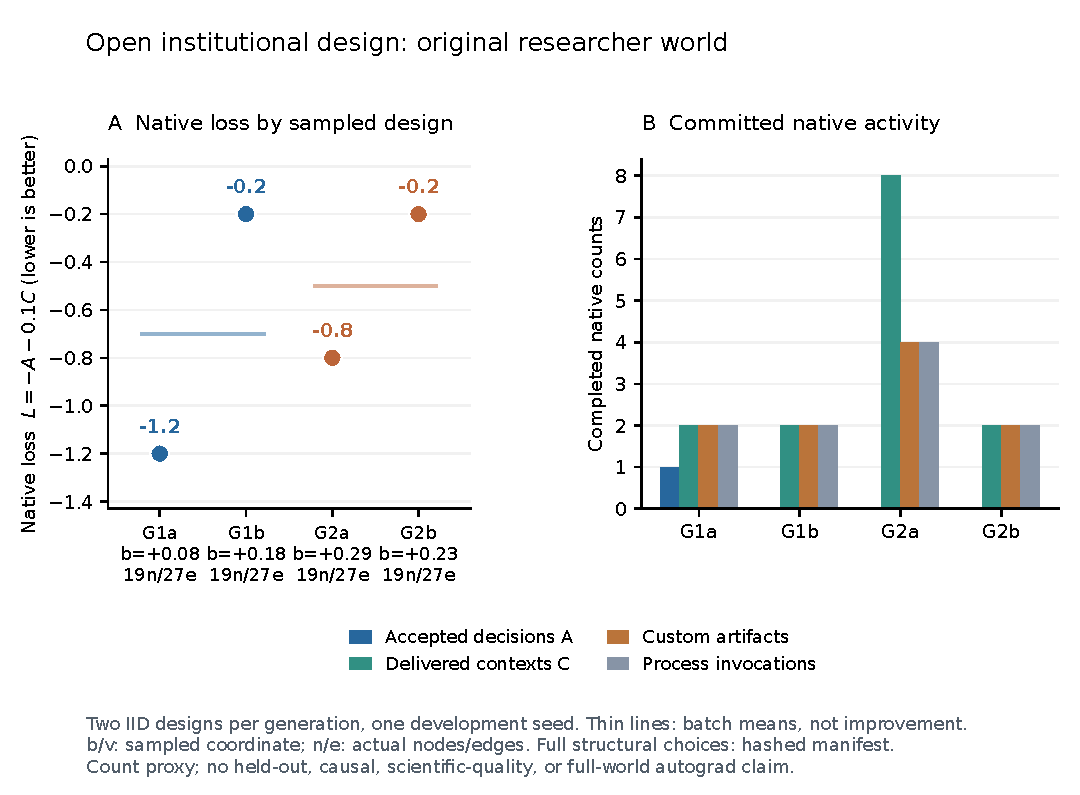
\includegraphics[width=\linewidth]{figures/native-open-v7.pdf}
\caption{Actual integrated open-native development probe. Each generation draws
two fresh systems with source-authored processes and a continuous coordinate.
The loss is the explicit engineering proxy $-A-0.1C$. Horizontal segments are
observed batch means, not estimates of improvement. The second generated source
does not beat the first observed incumbent. The bars show actual institutional
activity without interpreting more messages or artifacts as better science.
All nodes/edges remain 19/27; no topology invention is inferred from a source hash.}
\label{fig:open-native-v7}
\end{figure}
